\subsection{拉伸构建杯零件三维模型}
\begin{procedure}
\item 将大圆拉伸为圆柱。启动【拉伸】命令的方法有:
\begin{itemize}
\item 键盘输入EXTRUDE或EXT
\item 【绘图】菜单中【建模】子菜单中的【拉伸】项。
\item 单击【建模】工具栏中的【拉伸】图标
\includegraphics[scale=0.7]{extrudetool.png}。.
\end{itemize}
\begin{lstlisting}
|命令: EXTRUDE|
|当前线框密度:  ISOLINES=4,闭合轮廓创建模式 = 实体|
|选择要拉伸的对象或 [模式(MO)]: 找到 1 个\longremark{用拾取状态的鼠标选择最大的圆,选择后该圆会以虚线方式表示,如图\ref{fig:extrudeselecta}所示}|
|选择要拉伸的对象或 [模式(MO)]:|
|指定拉伸的高度或 [方向(D)/路径(P)/倾斜角(T)/表达式(E)]: -15\longremark{做拉伸操作是既可以使用正值,也可以使用负值,两者的区别拉伸的方向发生变化。在本例中拉伸的方向是由前向后拉伸。}|
\end{lstlisting}
\item 将小圆拉伸为圆柱。
\begin{lstlisting}
|命令: EXTRUDE|
|当前线框密度:  ISOLINES=4,闭合轮廓创建模式 = 实体|
|选择要拉伸的对象或 [模式(MO)]: 找到 1 个\longremark{用拾取状态的鼠标选取小圆做为拉伸对象,如图\ref{fig:extrudeselectb}所示,若再选择大圆将不能够选中,因为此时的大圆已经是一个实体。}|
|选择要拉伸的对象或 [模式(MO)]:|
|指定拉伸的高度或 [方向(D)/路径(P)/倾斜角(T)/|
|表达式(E)] $<-15.0000>$: -10|
\end{lstlisting}
\begin{figure}[htbp]
\centering
\subfloat[]{\label{fig:extrudeselecta}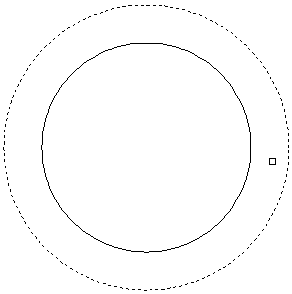
\includegraphics[scale=0.5]{extrudeselect.png}}\hspace{20pt}
\subfloat[]{\label{fig:extrudeselectb}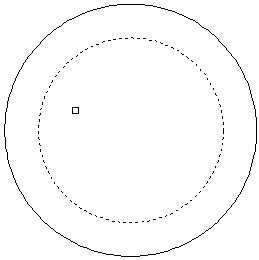
\includegraphics[scale=0.5]{extrudeselect1.png}}
\caption{拉伸过程}
\end{figure}
\showremarks
\item 将视图切换为【东南等轴测】。点击【视图】菜单中【三维视图】子菜单中的【东南等轴测】项。
\item 从大圆柱中减去小圆柱。要实现该操作需要用到实体编辑中的【差集】命令,其启动方法有:
\begin{itemize}
\item 键盘输入SUBTRACT或SU。
\item 【修改】菜单中【实体编辑】子菜单中的【差集】命令。
\item 单击【实体编辑】工具栏中的【差集】图标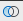
\includegraphics[scale=0.7]{subtracttool.png}。
\end{itemize}
\begin{lstlisting}
|命令: SUBTRACT |
|选择要从中减去的实体、曲面和面域...|
|选择对象: 找到 1 个\longremark{选择大圆柱做为要从中减去的实体,如图\ref{fig:subtractselect1}所示。}|
|选择对象:  选择要减去的实体、曲面和面域...|
|选择对象: 找到 1 个\longremark{选择小圆柱做为要减去的实体,如图\ref{fig:subtractselect2}所示。}|
|选择对象:|
\end{lstlisting}
\begin{figure}[htbp]
\centering
\subfloat[]{\label{fig:subtractselect1}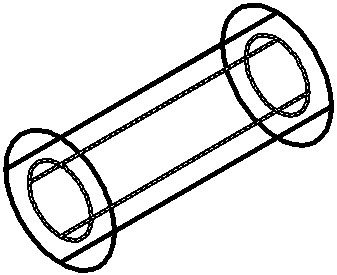
\includegraphics[scale=0.5]{subtractselect1.png}}\hspace{20pt}
\subfloat[]{\label{fig:subtractselect2}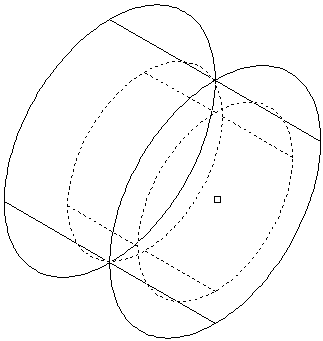
\includegraphics[scale=0.5]{subtractselect2.png}}
\caption{差集过程}
\end{figure}
\showremarks
\item 切换视觉样式为灰度。点击【视图】菜单中【视觉样式】子菜单中的【灰度】项。
\end{procedure}

通过上述步骤,我们获得了与图\ref{fig:beimodel}一样的三维模型。
\endinput